
\documentclass[12pt]{amsart}
\usepackage{geometry} % see geometry.pdf on how to lay out the page. There's lots.
\geometry{a4paper} % or letter or a5paper or ... etc
\usepackage[T1]{fontenc}
\usepackage[latin9]{inputenc}
\usepackage{amsmath}
\usepackage{amsaddr}
\usepackage{dirtytalk}
\usepackage{float}
\usepackage{listings}
\usepackage{hyperref}
\usepackage{enumerate}
\usepackage{graphicx}
\graphicspath{ {../support_files/} }

\usepackage{color}
 
\definecolor{codegreen}{rgb}{0,0.6,0}
\definecolor{codegray}{rgb}{0.5,0.5,0.5}
\definecolor{stringcolor}{rgb}{0.7,0.23,0.36}
\definecolor{backcolour}{rgb}{0.95,0.95,0.92}
\definecolor{keycolor}{rgb}{0.007,0.01,1.0}
\definecolor{itemcolor}{rgb}{0.01,0.0,0.49}

\hypersetup{
    colorlinks=true,
    linkcolor=blue,
    filecolor=blue,      
    urlcolor=blue,
}
 
\lstdefinestyle{mystyle}{
    %backgroundcolor=\color{backcolour},   
    commentstyle=\color{codegreen},
    keywordstyle=\color{keycolor},
    numberstyle=\tiny\color{codegray},
    stringstyle=\color{stringcolor},
    basicstyle=\footnotesize,
    breakatwhitespace=false,         
    breaklines=true,                 
    captionpos=b,                    
    keepspaces=true,                 
    numbers=left,                    
    numbersep=5pt,                  
    showspaces=false,                
    showstringspaces=false,
    showtabs=false,                  
    tabsize=2
}
 
\lstset{style=mystyle}

\lstdefinelanguage{Swift}{
  keywords={associatedtype, class, deinit, enum, extension, func, import, init, inout, internal, let, operator, private, protocol, public, static, struct, subscript, typealias, var, break, case, continue, default, defer, do, else, fallthrough, for, guard, if, in, repeat, return, switch, where, while, as, catch, dynamicType, false, is, nil, rethrows, super, self, Self, throw, throws, true, try, associativity, convenience, dynamic, didSet, final, get, infix, indirect, lazy, left, mutating, none, nonmutating, optional, override, postfix, precedence, prefix, Protocol, required, right, set, Type, unowned, weak, willSet},
  ndkeywords={class, export, boolean, throw, implements, import, this},
  sensitive=false,
  comment=[l]{//},
  morecomment=[s]{/*}{*/},
  morestring=[b]',
  morestring=[b]"
}

\lstset{emph={Int,count,abs,repeating,Array}, emphstyle=\color{itemcolor}}


\title{Week 09}

\date{\today}

\lstset{style=mystyle}

%%% BEGIN DOCUMENT
\begin{document}
\maketitle

\section{Preparation for Assignment}
If, and \textit{only if} you can truthfully assert the truthfulness of each statement below are you ready to start the exercises.
\subsection {Reading Comprehension Self-Check}
\begin{itemize}
\item I understand that the \textbf{greedy technique} suggests constructing a solution to an optimization problem through a sequence of steps, each expanding a partially constructed solution obtained so far, until a complete solution to the problem is reached.
 \item I know why it is \textbf{false} to say that on each step of a greedy algorithm, the choice made must be \textit{feasible, globally optimal, and irrevocable}.
 \item I know why it is \textbf{false} to say that Prim\textquoteright{}s and Kruskal\textquoteright{}s algorithms are two different greedy algorithms for constructing minimum spanning trees of weighted \textit{unconnected} graphs.
 \item I know why it is \textbf{false} to say that the problem of scheduling \textit{n} jobs of unknown durations for execution by a single processor is ideal for solution with a greedy algorithm.
 \item I have begun figuring out how a greedy algorithm can be used to find an optimal set of \textit{n} weights so that it would be possible to weigh on a balance scale any integer load in the largest possible range from $1$ to $W$, provided weights can be put only on the free cup of the scale, or provided weights can be put on both cups of the scale.
 \item I remember what a digraph is.
 \item I know that Dijkstra?s algorithm solves the single-source shortest-path problem of finding shortest paths from a given vertex (the source) to all the other vertices of a weighted graph or digraph.
 \item I know that Dijkstra\textquoteright{}s algorithm works like Prim?s algorithm but compares path lengths rather than edge lengths.
 \item I know why Dijkstra?s algorithm always yields a correct solution for a graph with nonnegative weights.
 \item I know that a Huffman tree is a binary tree that minimizes the weighted path length from the root to the leaves of predefined weights.
 \item I know that the most important application of Huffman trees is Huffman codes.
 \item I know that a Huffman code is an optimal prefix-free variable-length encoding scheme that assigns bit strings to symbols based on their frequencies in a given text.
 \item I know that a Huffman code is created by a greedy construction of a binary tree whose leaves represent the alphabet symbols and whose edges are labeled with 0?s and 1?s.
\end{itemize}
\subsection{Memory Self-Check}
How many algorithms for finding minimum spanning trees of undirected connected graphs, with their names, do you remember from the reading for this week? How many others, including their names, can you find on the internet?
 \section{Week 09 Exercises}
\subsection{ Exercise 1 on page 322}
Write code in a language of your choice instead of pseudocode. 
\subsection{Exercise 1 on page 332} 
\subsection{Exercise 2 on page 332} 
\subsection{Exercise 3 on page 338} 
\subsection{Exercise 1 on page 342} 
\subsection{Exercise 3 on page 343}


\section{Week 09 Problems}
\subsection{Exercise 3 on page 322}
\subsection{Not in the Book}

  Prim\textquoteright{}s and Kruskal\textquoteright{}s algorithms are quite similar. The only real difference is in the set of edges available for inclusion in the tree at each step. In Prim\textquoteright{}s algorithm, only those edges that are adjacent to edges already in the tree (and not completing simple cycles) may be added (so that, as a result, all the intermediate stages are trees). In Kruskal\textquoteright{}s algorithm, any edge that does not complete a simple cycle may be added (so that the intermediate stages may be forests and not trees). 
  
Create minimum spanning trees for each of these two graphs.

  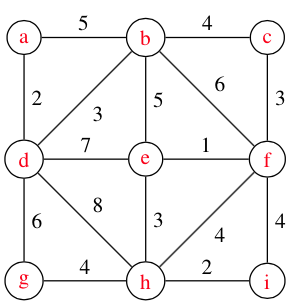
\includegraphics[scale=0.5]{mstgraph1}
  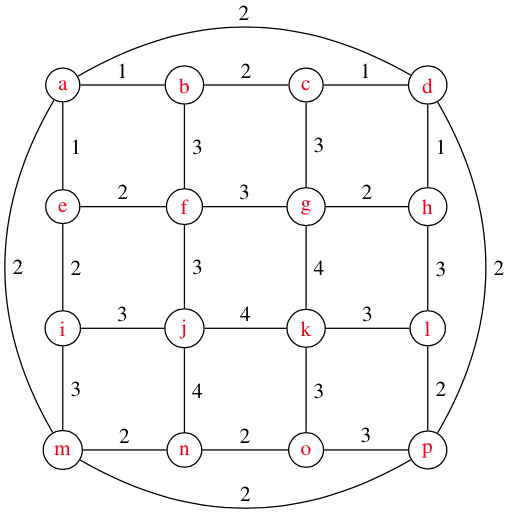
\includegraphics[scale=0.5]{mstgraph2}
When applicable, use lexicographical order to break ties. List the edges in the order chosen by each algorithm, and find the total weight.


  


\end{document}